\documentclass[parskip,a4paper]{scrartcl}
\usepackage[margin=15mm]{geometry}
\usepackage{tikz}

\begin{document}
\pagestyle{empty}

The following grid can be used to design \textbf{DUPLO compatible plates}. It
shows the basic $16$mm grid with nobs (diameter $9.6$mm) and build areas of
MakerBot Cupcake~CNC ($100\times 100$mm), Thing-O-Matic ($96\times 108$mm), and
Replicater ($145 \times 225$mm), and the smallest standard size of Ponoko (and
its partners RazorLAB, Formulor, and Vectorealism) ($181\times 181$mm).

\begin{tikzpicture}

\begin{scope}[dotted]
% duplo matrix
\draw[step=16mm] (0,0) grid (176mm,224mm);

% nops
\foreach \x [evaluate = \x as \xp using ((\x-0.5) * 16)] in {1,2,3,4,5,6,7,8,9,10,11}{
  \foreach \y [evaluate = \y as \yp using ((\y-0.5) * 16)] in {1,2,3,4,5,6,7,8,9,10,11,12,13,14}{
    \draw (\xp mm,\yp mm) circle (4.8mm);
  }
}
\end{scope}

% areas
\draw (0,0) rectangle (100mm,100mm);
\draw (0,0) rectangle (181mm,181mm);
\draw (0,0) rectangle (145mm,225mm);
\draw (0,0) rectangle (96mm,108mm);
\end{tikzpicture}

\pagebreak
\pagestyle{empty}

The bars should not be tight, so I choose make them $12$mm diameter (including an expected
$0.25$mm laser cutter width. Marble holes are $16$mm diameter and marble tracks $12$mm, so
marbles should have diameter between $13$ and $15$mm.

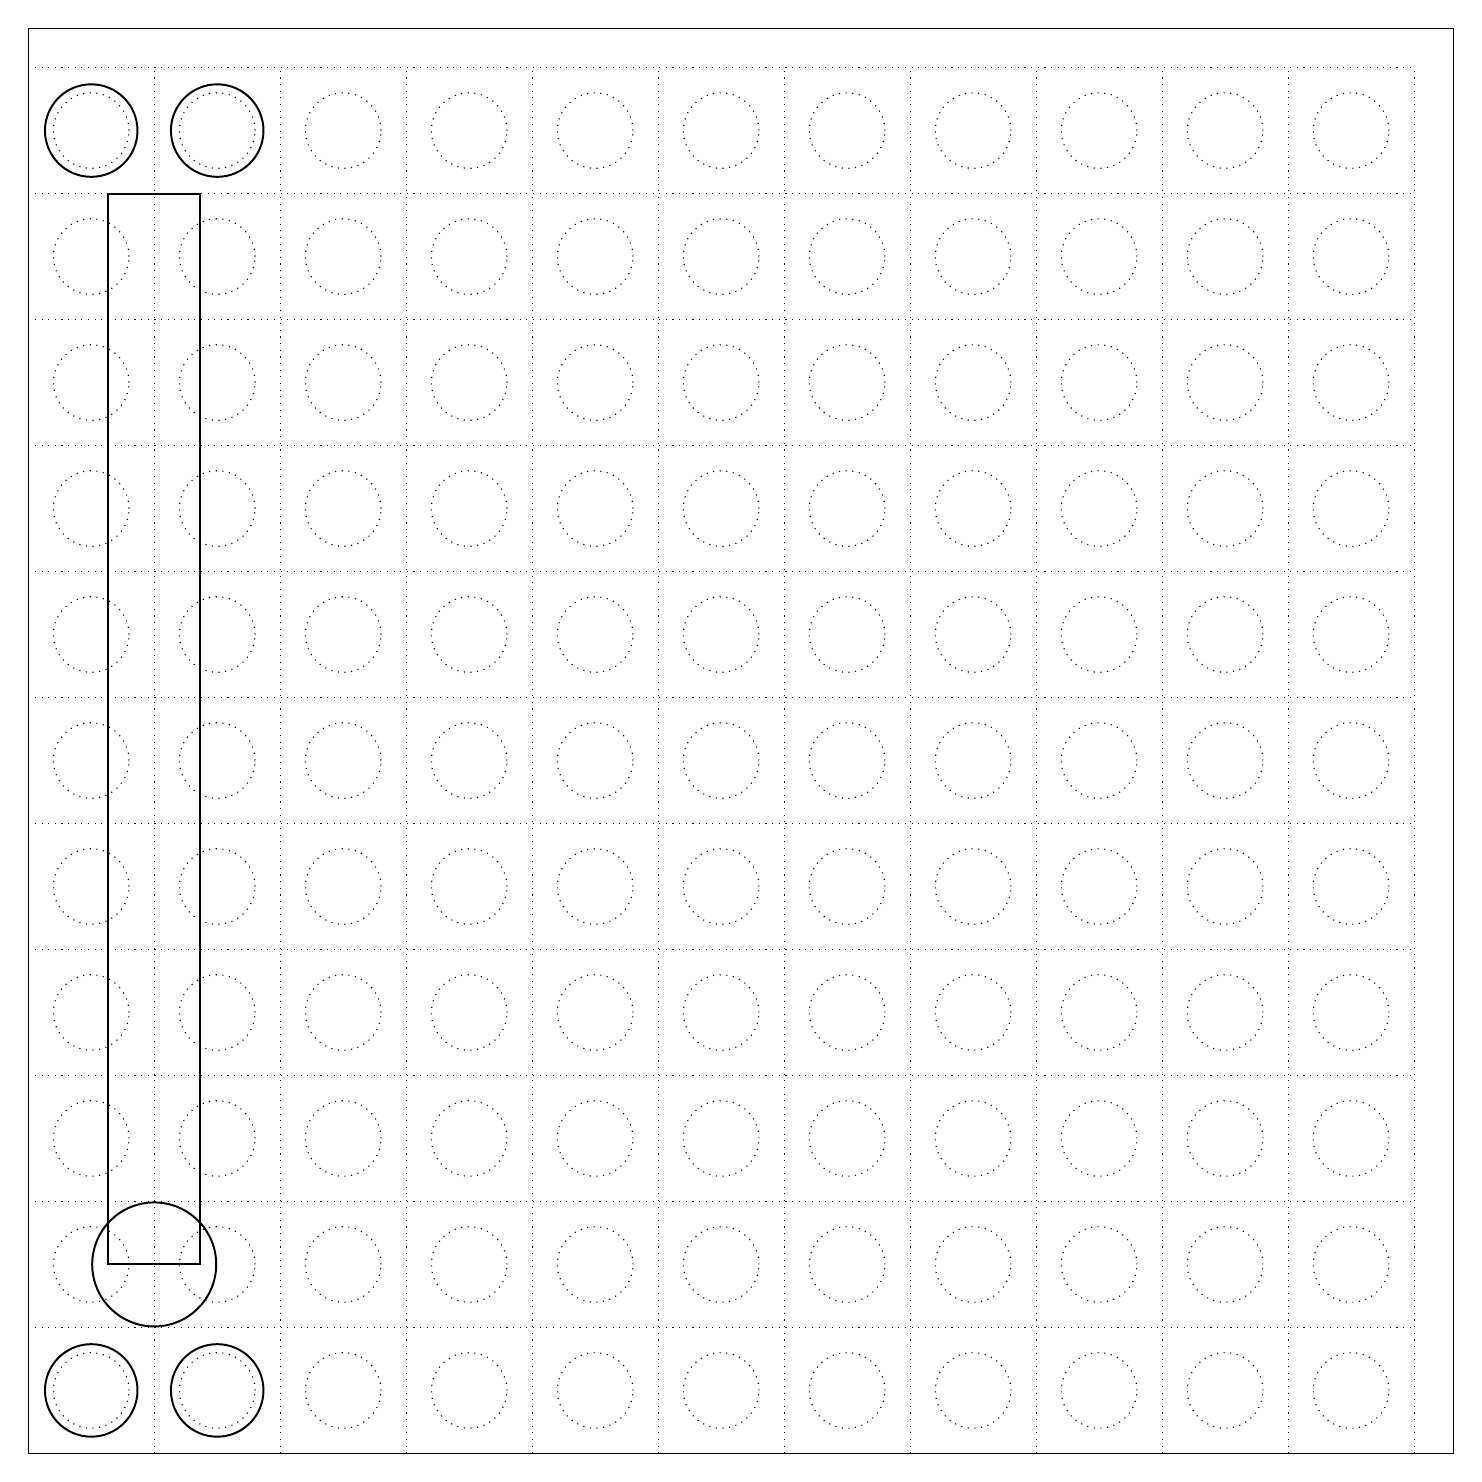
\begin{tikzpicture}
\draw[step=16mm,dotted] (0,0) grid (176mm,176mm);
\foreach \x [evaluate = \x as \xp using ((\x-0.5) * 16)] in {1,2,3,4,5,6,7,8,9,10,11}{
  \foreach \y [evaluate = \y as \yp using ((\y-0.5) * 16)] in {1,2,3,4,5,6,7,8,9,10,11}{
    \draw[dotted] (\xp mm,\yp mm) circle (4.8mm);
  }
}
\draw (0,0) rectangle (181mm,181mm);

\foreach \x [evaluate = \x as \xp using ((\x-0.5) * 16)] in {1,2}{
  \foreach \y [evaluate = \y as \yp using ((\y-0.5) * 16)] in {1,11}{
    \draw[line width=0.25mm] (\xp mm,\yp mm) circle (5.875mm);
  }
}

\begin{scope}[line width=0.25mm]
\draw (10.125mm,24mm) rectangle (21.875mm,160mm);
\draw (16mm,24mm) circle (7.875mm);
\end{scope}

% line width=0.25mm
%expected cutting/layer width: $0.25$mm.
\end{tikzpicture}

\end{document}
